\documentclass{article}
\title{Belousov-Zhabotinskii Reaction}
\author{Zachariah Sachs (with Jeff Montgomery)}
\usepackage{graphicx}
\usepackage{float}
\usepackage{IEEEtrantools}
\usepackage{textcomp}
\usepackage{fixltx2e}

\begin{document}
\maketitle
\section{Purpose}

In this laboratory exercise, we explore the oscillatory kinetics manifest in temporal and
spatial complexity of the Belousov-Zhabotinskii reaction through analysis of spectral data 
over time for the seemingly homogeneous three-dimensional process and of wave 
propagation in the inhomogeneous thin-layer two-dimensional case.

\section{Theory and Methods}

\subsection{Complexity, Oscillations, and the Lotka Mechanism}

Many important processes in biology and elsewhere depend on dynamic behavior which does 
not proceed monotonically toward equilibrium and which is sensitive to spatial 
inhomogeneities and concentration gradients. Really, any cyclic biochemical process, such as
glycolysis in yeast, must respond to the chemical environment to fulfill the needs of a living 
organism. These reactions must not overconsume resources or overproduce products, yet a
nonzero chemical potential is necessary to do work. Complexities
may be localized to a single cell, as in the self-replication of RNA, or coordinated through a 
much larger organism, as needed to maintain the regular beating of a heart. Obviously, these
chemical processes must provide amplification and feedback in the right location and on an
appropriate timescale to function properly.

Alfred Lotka hypothesized the following set of reactions which would show temporal
oscillations of intermediates $X$ and $Y$ in the overall reaction $A\longrightarrow P$:
\begin{IEEEeqnarray}{rcl}
A+X & \stackrel{k_1}{\longrightarrow} & 2X \\
X+Y & \stackrel{k_2}{\longrightarrow} & 2Y \\
Y     & \stackrel{k_3}{\longrightarrow} & P.
\end{IEEEeqnarray}
Reactions (1) and (2) are autocatalytic, and reactions (2) and (3) use reactants from (1) and (2)
to provide negative feedback. The rate equations for this system are then
\begin{IEEEeqnarray}{rcl}
\frac{d[A]}{dt} & = & -k_1[A][X] \\
\frac{d[X]}{dt} & = & k_1[A]-k_2[X][Y] \\
\frac{d[Y]}{dt} & = & k_2[X][Y]-k_3[Y] \\
\frac{d[P]}{dt} & = & k_3[Y].
\end{IEEEeqnarray}
These differential equations are nonlinear as a result of the feedback in the system, and 
complexity in the form of oscillations will likely result.

\subsection{The Field-K\"or\"os-Noyes Mechanism for the Belousov-Zhabotinskii Reaction}

The Belousov-Zhabotinskii (BZ) reaction was discovered by Belousov, reproduced by 
Zhabotinskii, and a model for its mechanism was proposed by Field, K\"or\"os, and Noyes.
In a well-stirred solution, the three-dimensional case, the electrochemical potential 
oscillates displaying homogeneous color changes as the reaction cycles. In unstirred 
solution, the two-dimensional case, diffusion of reaction intermediates produces spatial 
concentration  gradients which propogate and are visible as a color wave.

Like the Lotka Mechanism, concentrations of the intermediates in the  BZ reaction oscillate
as the concentration of the products proceeds to equilibrium. Bromine-containing 
intermediates and cerium(III/IV) catalysts aid in the overall oxidation by bromate,
BrO\textsubscript{3}\textsuperscript{-}, of malonic acid,
CH\textsubscript{2}(COOH)\textsubscript{2}, to carbon dioxide, water, and bromide. The
Field-K\"or\"os-Noyes (FKN) mechanism for the BZ reaction involves nine key steps and 
includes feedback and autocatalysis\footnote{The key reactions of the FKN mechanism, 
included in  the procedure, are suppressed here.}. The FKN mechanism is simplified in the 
``Oregonator'' scheme,
\begin{IEEEeqnarray}{rcl}
A+Y & \stackrel{k_1}{\longrightarrow} & X \\
X+Y & \stackrel{k_2}{\longrightarrow} & P \\
B+X & \stackrel{k_3}{\longrightarrow} & 2X+Z \\
2X   & \stackrel{k_4}{\longrightarrow} & Q \\
Z     & \stackrel{k_5}{\longrightarrow} & Y,
\end{IEEEeqnarray}
where $A=B$=BrO\textsubscript{3}\textsuperscript{-} is substrate, 
$X$=HBrO\textsubscript{2}, $Y$=Br\textsuperscript{-}, and $Z$=Ce\textsuperscript{4+} are
intermidiates, and P and Q are products.
Note equation (10) is coupled to the other four equations; it appears to be the crux of 
feedback in this system, and is also the only autocatalytic step. This mechanism is clearly
more complex than the Lotka mechanism, and therefore could either have more controlled
or more chaotic behavior.
The kinetics for this system are then given by the
differential equations
\begin{IEEEeqnarray}{rcl}
\frac{d[X]}{dt} & = & k_1[A][Y]-k_2[X][Y]+k_3[B][X]-2k_4[X]^2 \\
\frac{d[Y]}{dt} & = & -k_1[A][Y]-k_2[X][Y]+k_5[Z] \\
\frac{d[Z]}{dt} & = & k_3[B][X]-k_5[Z].
\end{IEEEeqnarray}
Solutions to these differential equations will give the time-dependence of the concentration
of intermediates. If we consider the reaction initiated at a single point by a metal ion
catalyst, the diffusion of the reduced bromine-containing intermediates down their 
respective concentration gradients shows spatial dependence that results in a ``target 
pattern''.

\subsection{Procedure}

\subsubsection{Stirred BZ Reaction (3-D)}

Initially, 5 mL each of 1.5 M sodium bromate and 0.25 M sodium bromide were mixed in a 
beaker on a stir plate. A stir bar was spun to produce a vortex in the solution, to which
5 mL each of 1.5 M malonic acid and 0.03 M cerium(IV) ammonium nitrate in 1.76 M sulfuric 
acid were
supposed\footnote{Both the 0.03 M cerium(IV) ammonium nitrate in 1.76 M 
sulfuric acid intended for the three-dimensional reaction and the plain 1.76 M sulfuric acid
intended for the two-dimensional reaction were labelled ``Solution D''. We confused the 
latter for the former here. Though we finished collecting data on our mistake with time to 
spare, computer malfunctions prevented us from collecting spectral data on the correct 
reaction. Our analysis will be adjusted accordingly}
to be added. After an amber color from the production of bromine faded, leaving a colorless 
solution, 200 $\mu$L of 0.025 M ferroin was added.
The initial concentrations of the components of this mixture are then 0.375 M 
bromate, 0.0625 M bromide, 0.375 M malonic acid, 0.0075 M cerium(IV) cations, 0.44 M 
hydronium, and 0.25 mM ferroin.
We eyed the mixture and observed quick 
flashes of green to blue-violet punctuating a predominate red color.

Spectral measurements were taken with an Ocean Optics model USB4000 spectrometer and
an LS-1 light source controlled by the SpectraSuite program, with integration time 60 ms, 
boxcar width 5, and scans to average 5. We continued to stir the reaction solution 
thourghout these measurements. First we collected a strip chart of the absorption at
415 nm, 520 nm, and 605 nm every 0.5 s for about 5 minutes. Then we set the computer
to save spectra at regular intervals and collected 101 different absorption spectra.

\subsubsection{Thin-Layer (2-D) BZ Reaction}

Initially, 2.5 mL each of 1.5 M sodium bromate, 0.25 M sodium bromide, 1.5 M malonic acid,
and 1.76 M sulfuric acid were stirred in a beaker until the amber color from the production of 
bromine faded, leaving a colorless solution. To this a drop of 0.1\% Triton X-100 detergent
solution was added to facilitate spreading in a dish. Finally, 2 mL of 0.025 M ferroin was 
added. The initial concentrations of the components of this mixture are then 0.3125 M 
bromate, 0.052 M bromide, 0.3125 M malonic acid, 0.367 M hydronium, and 4.17 mM ferroin.
This solution was poured into a thin layer covering the bottom of a petri dish. The
BZ reaction was initiated by carefully dippng a piece of silver wire in at a point. A blue dot
was observed at that point, which then spread into a ``target pattern''.

A Zeiss Telaval inverted microscope, with a 6V/30W tungsten-halogen illuminator 
passed through a 488$\pm$10  nm Thorlabs FL488-10 interference filter and a 5X achromat
objective, was focused so the field of view was of order as wide as the distance between
``target'' bands. The illumination was adjusted to distinguish between the red (488 nm green 
light absorbed leaving a dark image), and blue (green light transmitted giving a light image) 
bands of the ``target''. More than 5000 frames of high  (1280x1024) resolution  black and 
white video of this focus  was recorded to a computer using a CMOS (Thorlabs DCC1545M) 
video camera and the uc480 Viewer program.

The resulting video file was analysed using the ImageJ program. The frames were stacked
on top of each other, and two circular areas, A and B, along the direction of propagation (in 
this case the Y direction through B then A) of the BZ wave were selected. The program 
measured the X and Y 
center of mass weighted with respect to the greyscale coloring of each circular area for each 
frame and returned a file with these data.

\section{Data and Plots}

\subsection{Stirred BZ Reaction (3-D)}

\subsubsection{Kinetics}

The absorption time series for the cerium catalyzed bulk BZ reaction is included below in 
Figure \ref{tscat}. This is the data obtained using a solution of 0.03 M cerium(IV) ammonium 
nitrate in 1.76 M sulfuric acid in accordance with the procedure.

\begin{figure}[H]
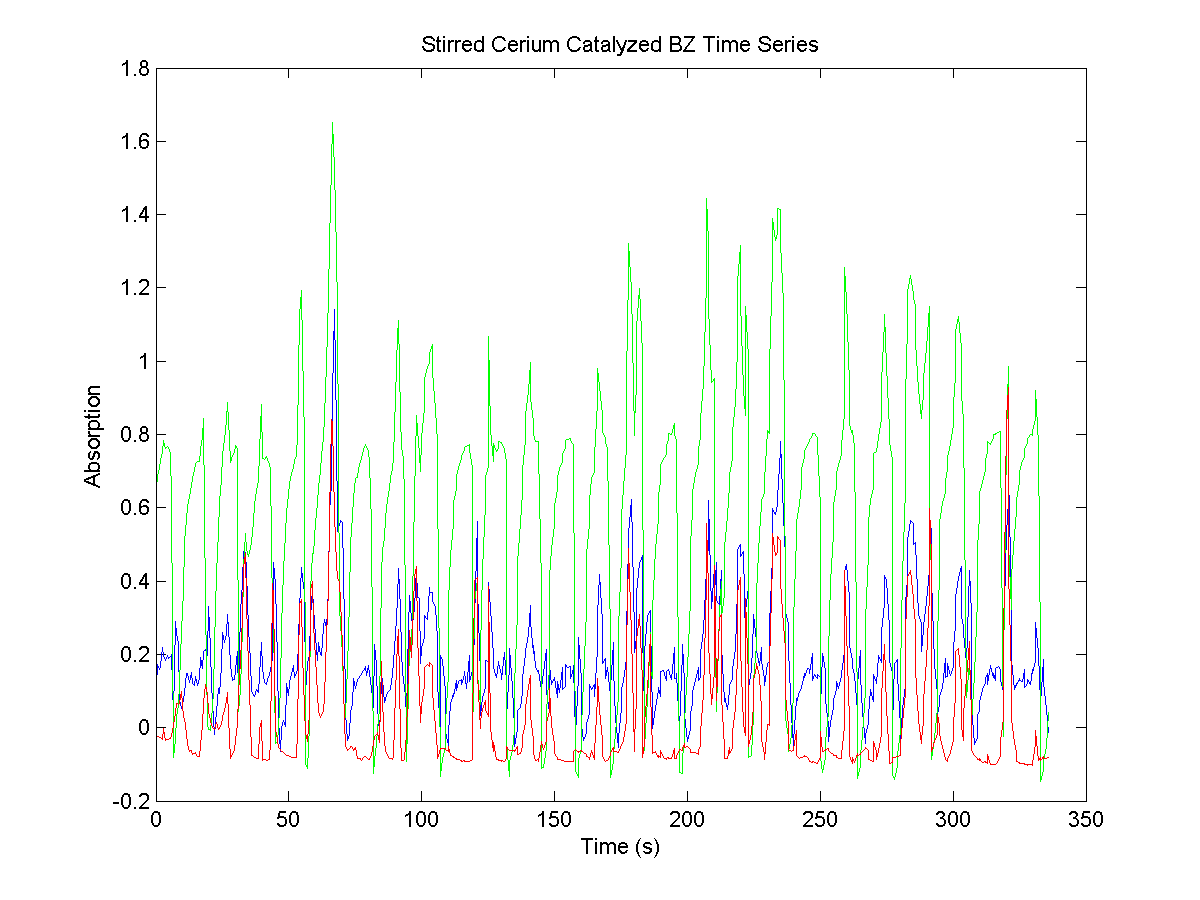
\includegraphics[width=0.8\textwidth]{TS}
\centering
\caption{Absorption time series for the cerium catalyzed bulk BZ reaction for 415 nm 
(blue), 520 nm (green), and 605 nm (red) light.}
\label{tscat}
\end{figure}

The absorption time series for the bulk BZ reaction without the cerium catalyst is included 
below in Figure \ref{tsun}. This is the data obtained using only 1.76 M sulfuric acid. Since 
this data is much less noisy, and since we were unable to obtain limiting spectra for the 
catalyzed reaction, we will continue our analysis with this data.

\begin{figure}[H]
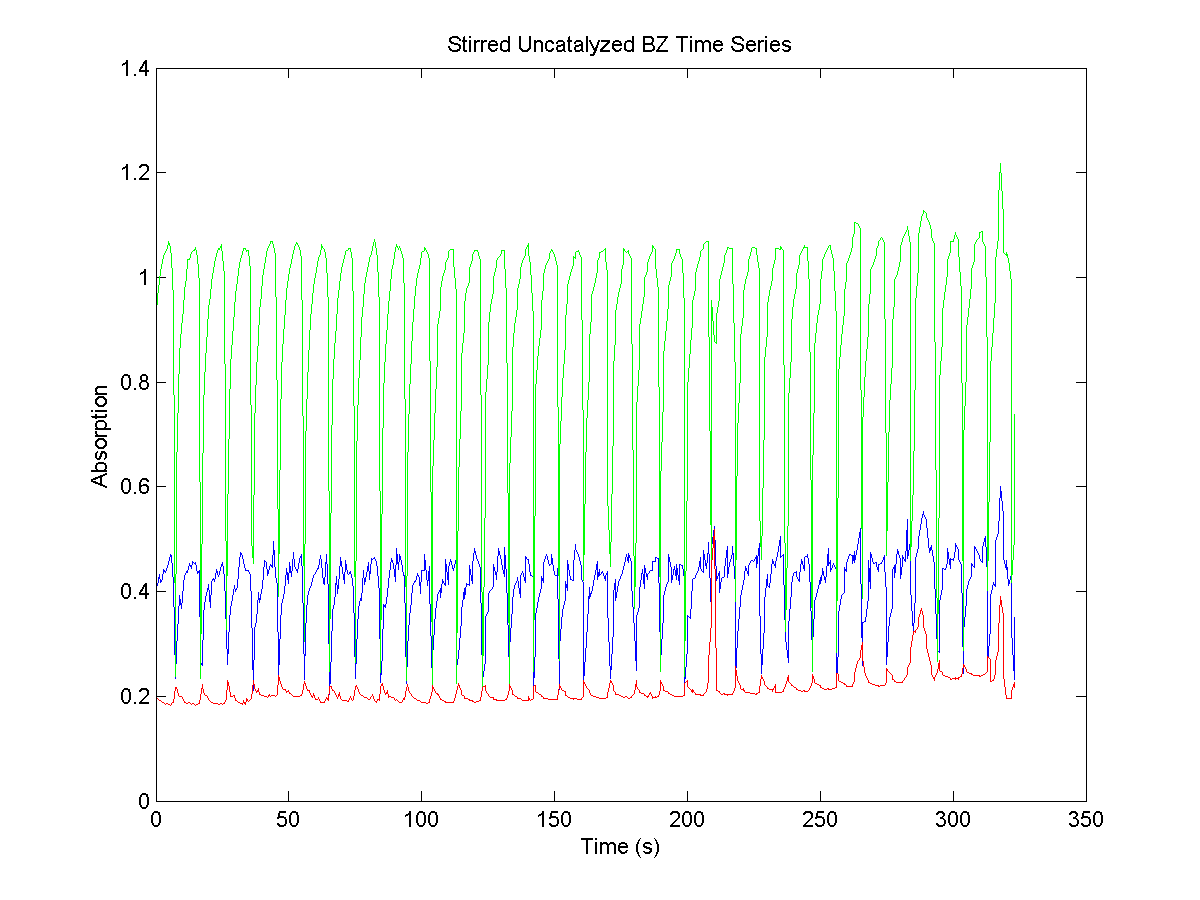
\includegraphics[width=0.8\textwidth]{TW}
\centering
\caption{Absorption time series for the uncatalyzed bulk BZ reaction for 415 nm 
(blue), 520 nm (green), and 605 nm (red) light.}
\label{tsun}
\end{figure}

\subsubsection{Unique Absorption Spectra}

The primary colors visible in the bulk reaction were long periods of red interspersed with
rapid flashes of aquamarine. These
transmitted colors correspond to the absorption of green light and red light, respectively.
It was suggested to me that the purpose of the cerium catalyst was to slow the oscillations
of the reaction. Looking at the time series for the uncatalyzed reaction above in Figure
ref{tsun}, it is clear that the maximum absorption for red light is much lower than the 
maximum absorbance for green light. Therefore, we expect the limiting spectra, that is those
for the unique appearances of red and aquamarine, to show an absorption peak around
500 nm for red, and a small peak, if any, above 600 nm for aquamarine. Of course, this
assumes the reactions oscillate with the same frequency and that we were able to capture
the spectra at the perfect time during the aquamarine flash. We can't assume.
The unique spectra are included below as Figures \ref{spr} and \ref{spaq}, respectively.

\begin{figure}[H]
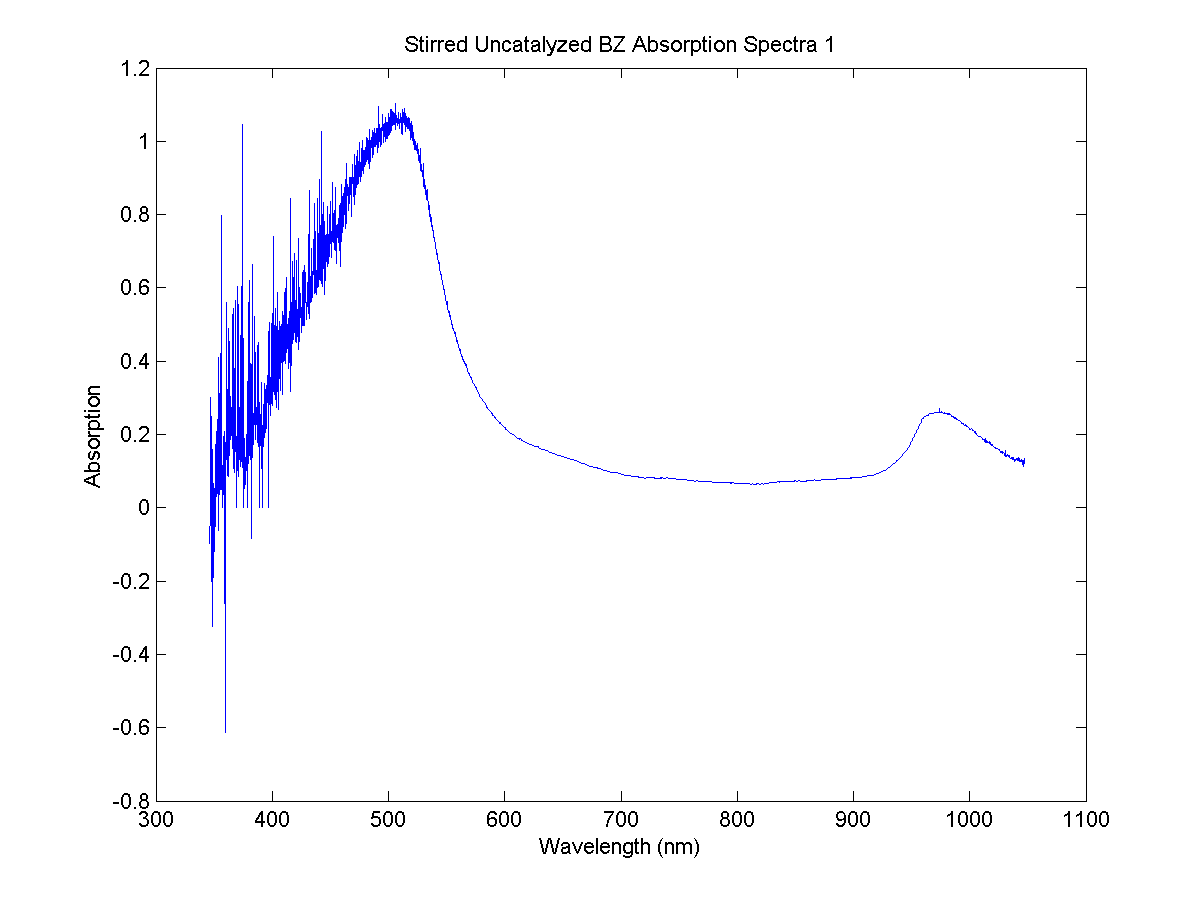
\includegraphics[width=0.8\textwidth]{sp001}
\centering
\caption{Limiting absorption spectra for the uncatalyzed bulk BZ reaction while appearing
 red.}
\label{spr}
\end{figure}

\begin{figure}[H]
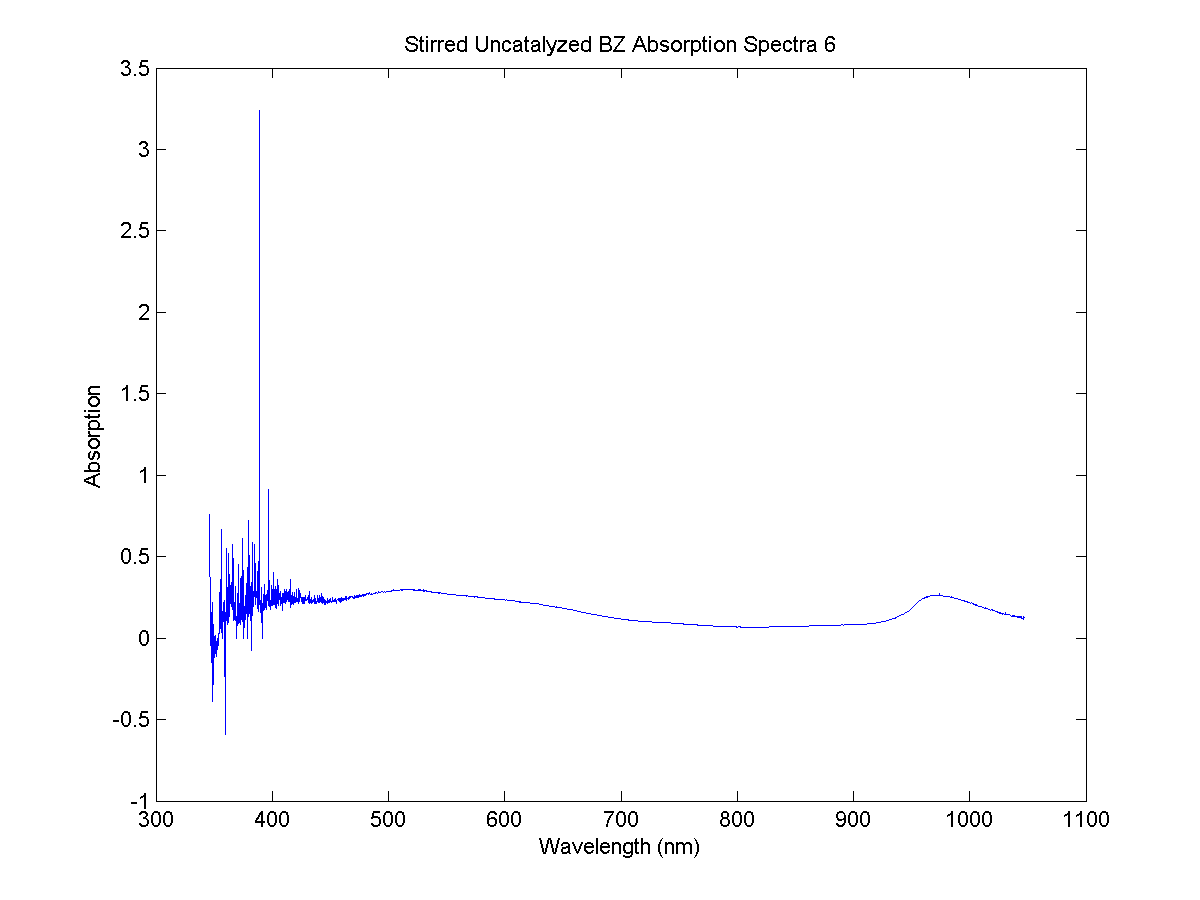
\includegraphics[width=0.8\textwidth]{sp006}
\centering
\caption{Limiting absorption spectra for the uncatalyzed bulk BZ reaction while appearing
aquamarine. }
\label{spaq}
\end{figure}

\subsection{Thin-Layer (2-D) BZ Reaction}

\subsubsection{Observations}

The reaction wavefronts were seen to reflect off of the walls of the container. Given how 
slowly the wavefronts progressed, we were not really able to see the reaction cease or the
thin-layer to homogenize. When we tried to do the reaction a second time, the reaction 
appeared to initiate on its own. This is likely the cause of residual silver left when we simply 
placed the wire in the second petri dish. I guess the silver necessary to initiallize the reaction
is minimal. We did not collect video of this second reaction dish.

\subsubsection{Frame Rate and Pixel Resolution}

The video recorded was 402 seconds long and had 5618 frames, giving an average frame rate 
of 13.98 frames per second.

CMOS camera images in the focal plane of the 5X objective have a resolution calibrated to
3.85 pixels per $\mu$m.

\subsubsection{Center of Mass}

The calculated Y-direction center of mass data for circular areas A and B, adjusted by a 
constant for clarity and divided by the pixel resolution to give a displacement, and with the 
frame count vector divided by the frame rate to give time, is included below in
Figure \ref{com}.

\begin{figure}[H]
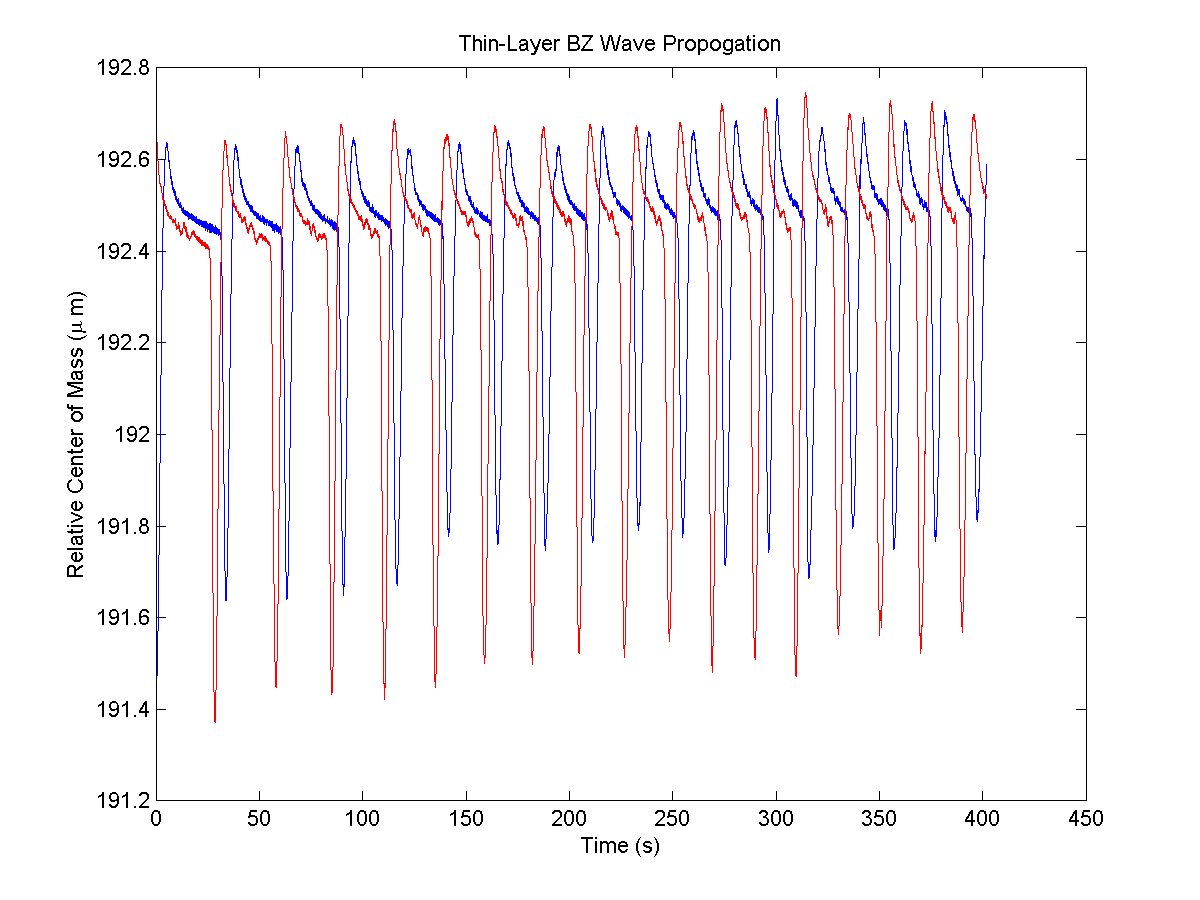
\includegraphics[width=0.8\textwidth]{comy}
\centering
\caption{Relative center of mass of circular areas A (blue) and B (red) over time in thin layer
BZ reaction.}
\label{com}
\end{figure}

\section{Analysis}

\subsection{Lotka Mechanism Simulation}

\subsubsection{Numerical Solutions}

Setting the constants $k_1$=0.01, $k_2$=0.03 and $k_3$=0.02 (all in units of
sec\textsuperscript{-1} M\textsuperscript{-1}), and
$[\mathrm{A}(0)]$=$[\mathrm{X}(0)]$=$[\mathrm{Y}(0)]$=1.0 M
and $[\mathrm{P}(0)]$=0.0 M in the
Lotka Mechanism, we solve the system of Equations (4) through (7) numerically. The result
is plotted below in figure \ref{losim}. Note that since we cannot solve the system analytically,
the plots below may only be of approximations that get worse the farther we look from our 
starting point.

\begin{figure}[H]
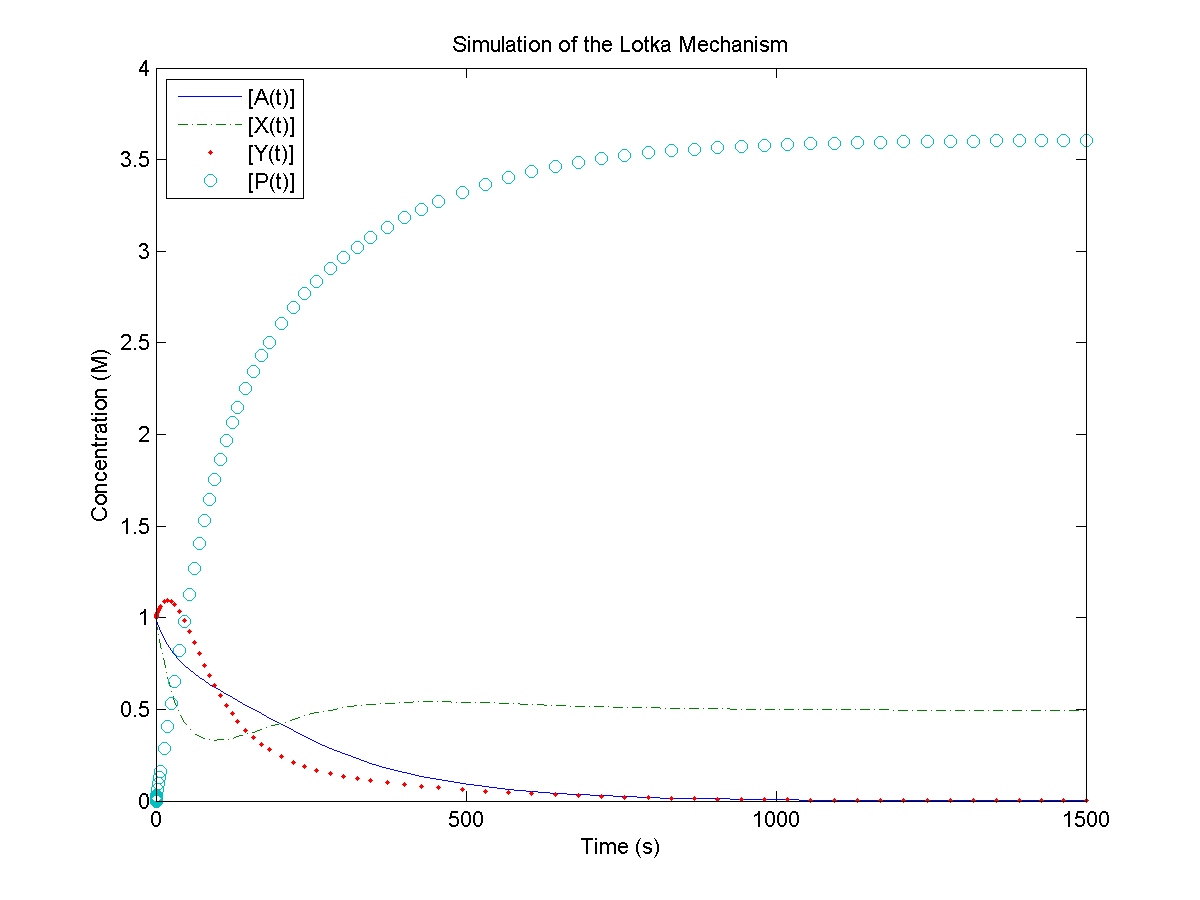
\includegraphics[width=0.8\textwidth]{LotkaSim}
\centering
\caption{Time dependence of concentrations of the four species in the Lotka Mechanism.}
\label{losim}
\end{figure}

\subsubsection{Fourier Transform Analysis}

The power spectra for the intermediates X and Y are included below in Figures \ref{frlx} and 
\ref{frly}. Considering the quality and quantity of simulated data available from an 
approximate numerical solution, these spectra are not particularly dense or distinct. They do
not show any predominant frequencies. Perhaps if the rate constants and initial conditions
were adjusted, or if we used a different solution method, we might get more obvious 
oscillations.

\begin{figure}[H]
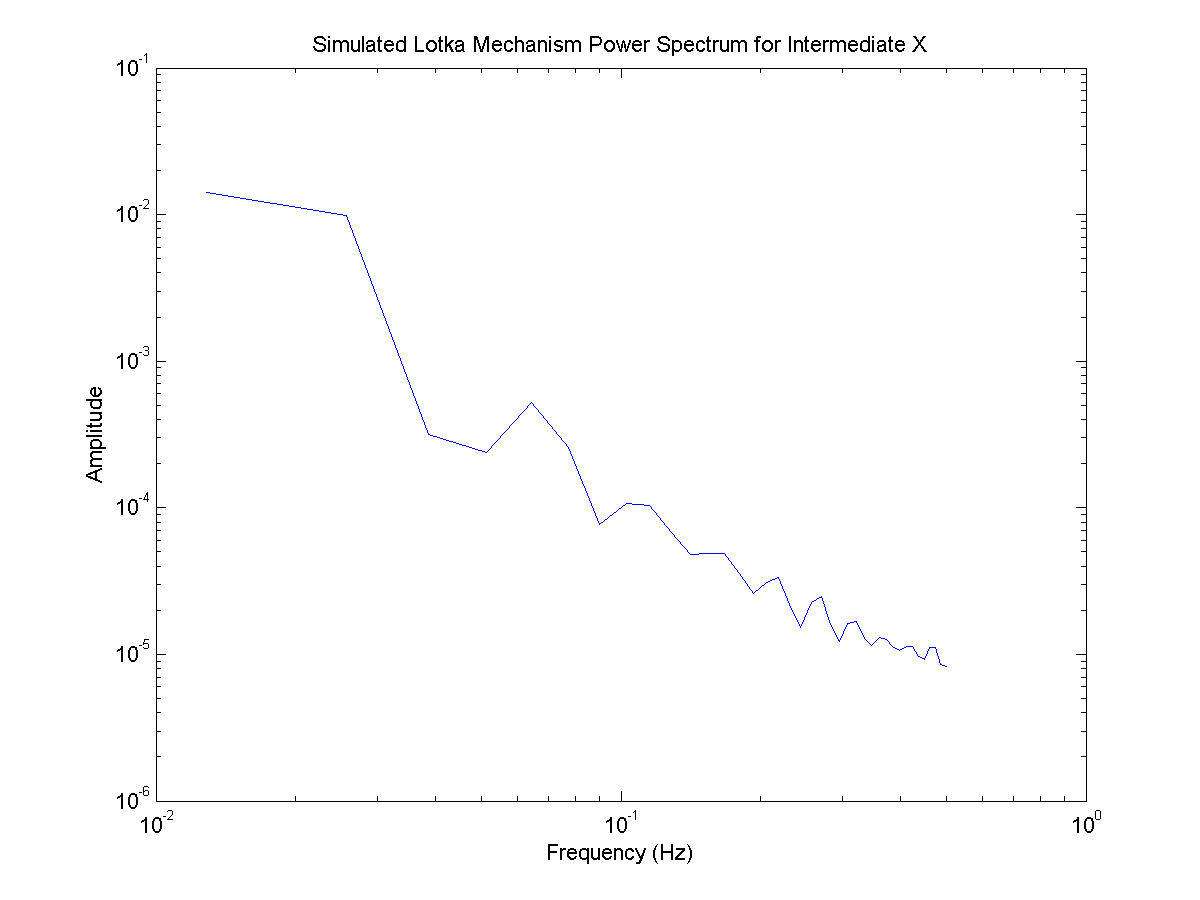
\includegraphics[width=0.8\textwidth]{fxpx}
\centering
\caption{Power spectrum of the concentrations of the intermediate X in the Lotka 
Mechanism.}
\label{frlx}
\end{figure}

\begin{figure}[H]
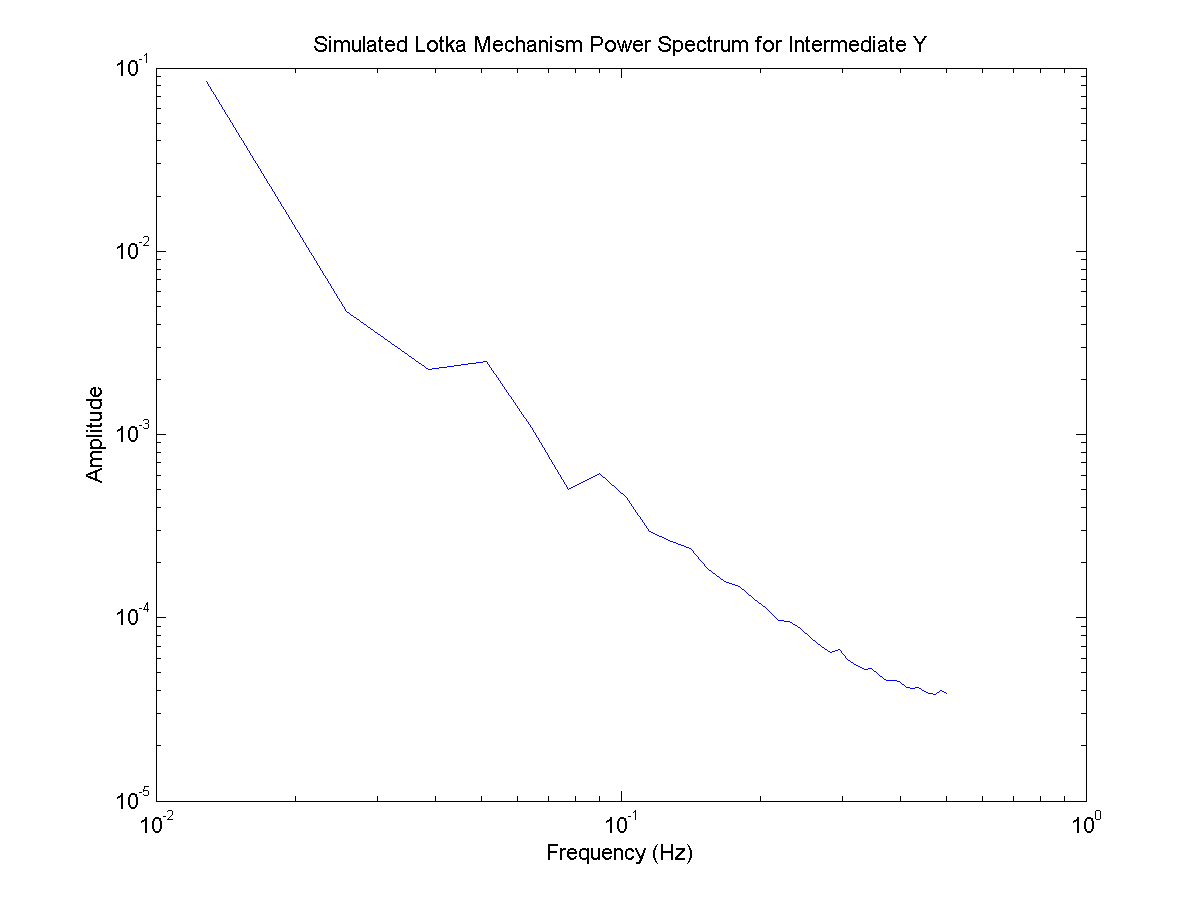
\includegraphics[width=0.8\textwidth]{fypy}
\centering
\caption{Power spectrum of the concentrations of the intermediate Y in the Lotka 
Mechanism.}\label{frly}
\end{figure}

\subsection{Stirred BZ Reaction (3-D)}

\subsubsection{Fourier Transform Analysis of the Cerium Catalyzed Reaction}

The power spectra of the time series for the cerium catalyzed bulk BZ reaction at all three
wavelengths are included below in Figures \ref{ftcat415}, \ref{ftcat520}, and \ref{ftcat605}.
The power spectrum in Figure \ref{ftcat520} shows the most obvious irregular spikes, which
have been marked with red circles. Notice that the amplitude appears to decrease linearly 
over regular frequency intervals on a log-log scale. Other than this, the cerium catalysed
power spectra are fairly indistinct.

\begin{figure}[H]
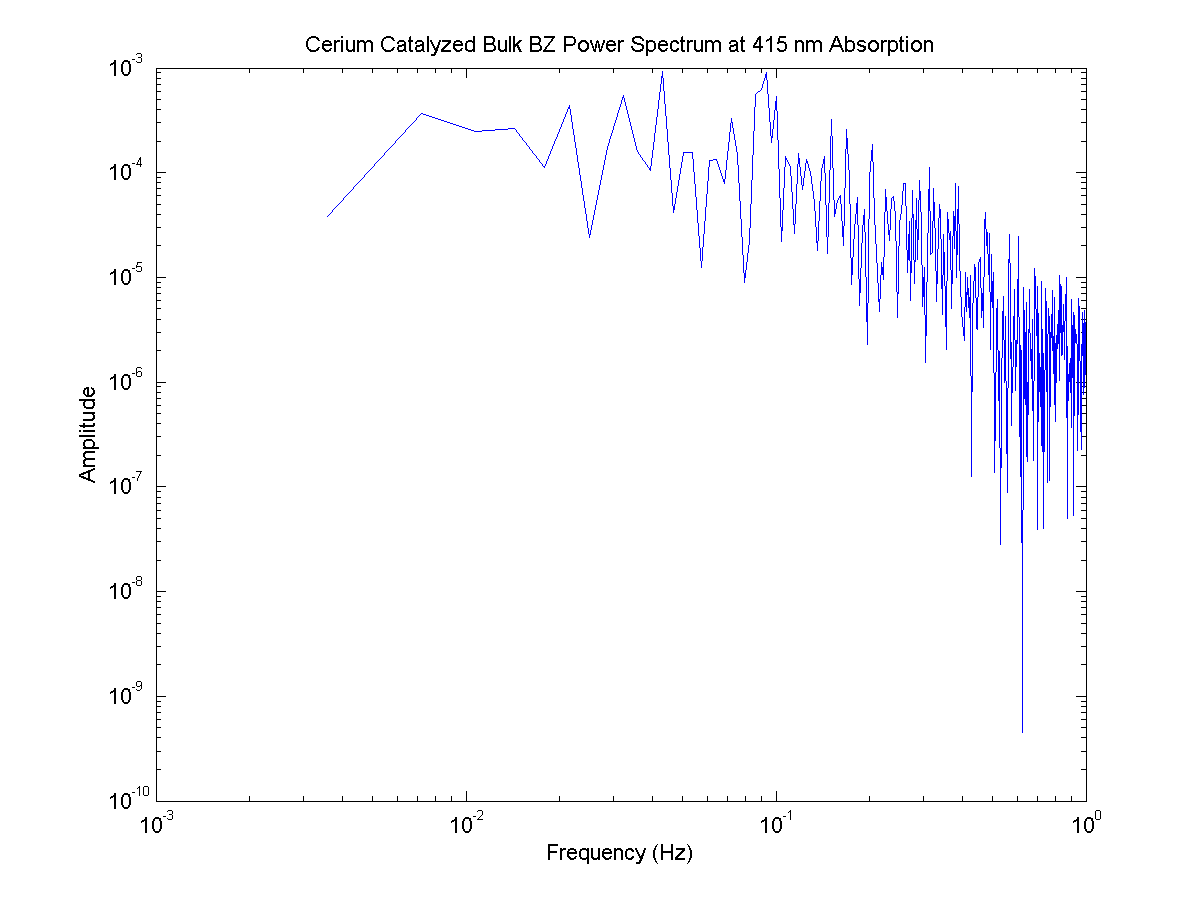
\includegraphics[width=0.8\textwidth]{frCe415}
\centering
\caption{Power spectrum of the 415 nm time series for the cerium catalysed bulk BZ 
reaction.}
\label{ftcat415}
\end{figure}

\begin{figure}[H]
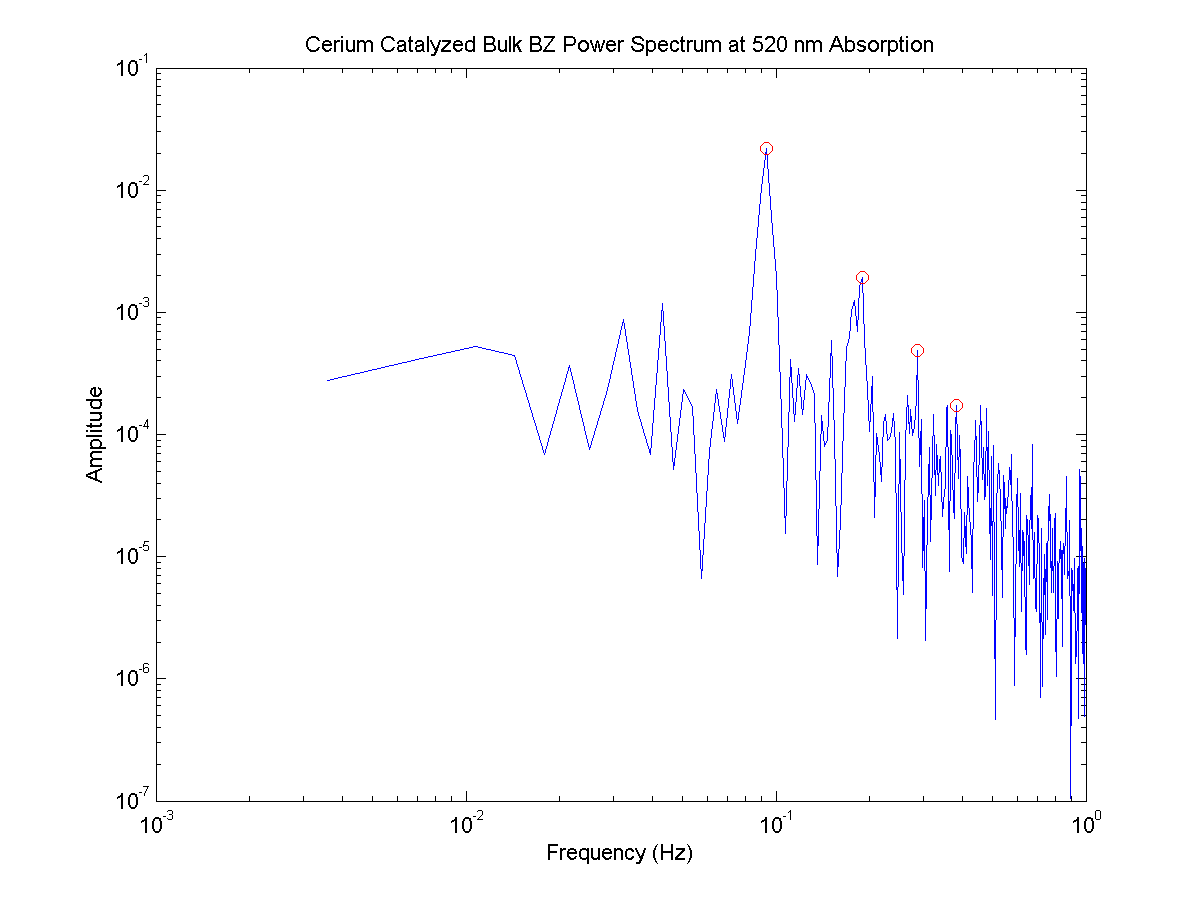
\includegraphics[width=0.8\textwidth]{frCe520}
\centering
\caption{Power spectrum of the 520 nm time series for the cerium catalysed bulk BZ 
reaction with irregular spikes marked.}
\label{ftcat520}
\end{figure}

\begin{figure}[H]
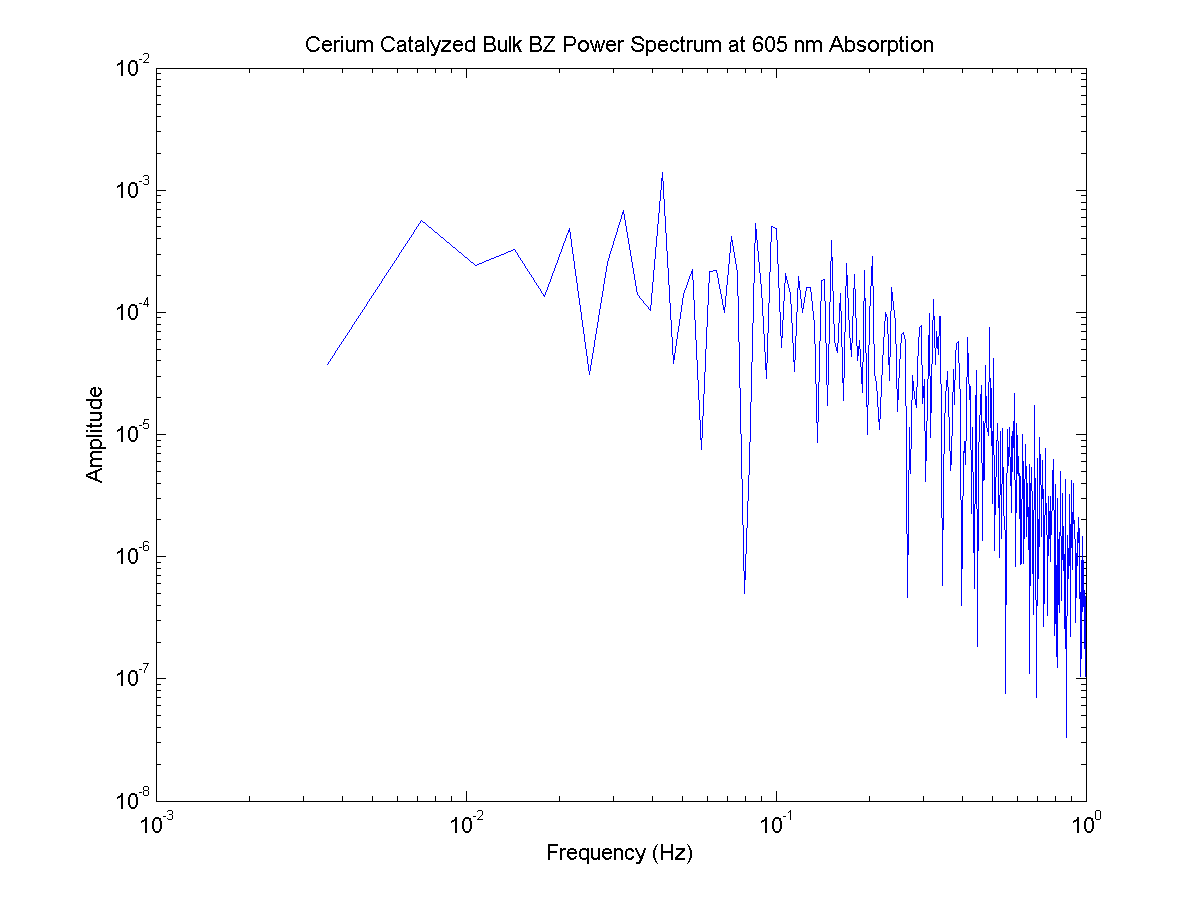
\includegraphics[width=0.8\textwidth]{frCe605}
\centering
\caption{Power spectrum of the 605 nm time series for the cerium catalysed bulk BZ 
reaction.}
\label{ftcat605}
\end{figure}

\subsubsection{Fourier Transform Analysis of the Uncatalyzed Reaction}

The power spectra of the time series for the uncatalyzed bulk BZ reaction at all three
wavelengths are included below in Figures \ref{ftw415}, \ref{ftw520}, and \ref{ftw605}.
All show obvious irregular spikes, which have been marked with red circles. Again, the 
amplitude appears to decrease linearly over regular frequency intervals on a log-log scale. 

\begin{figure}[H]
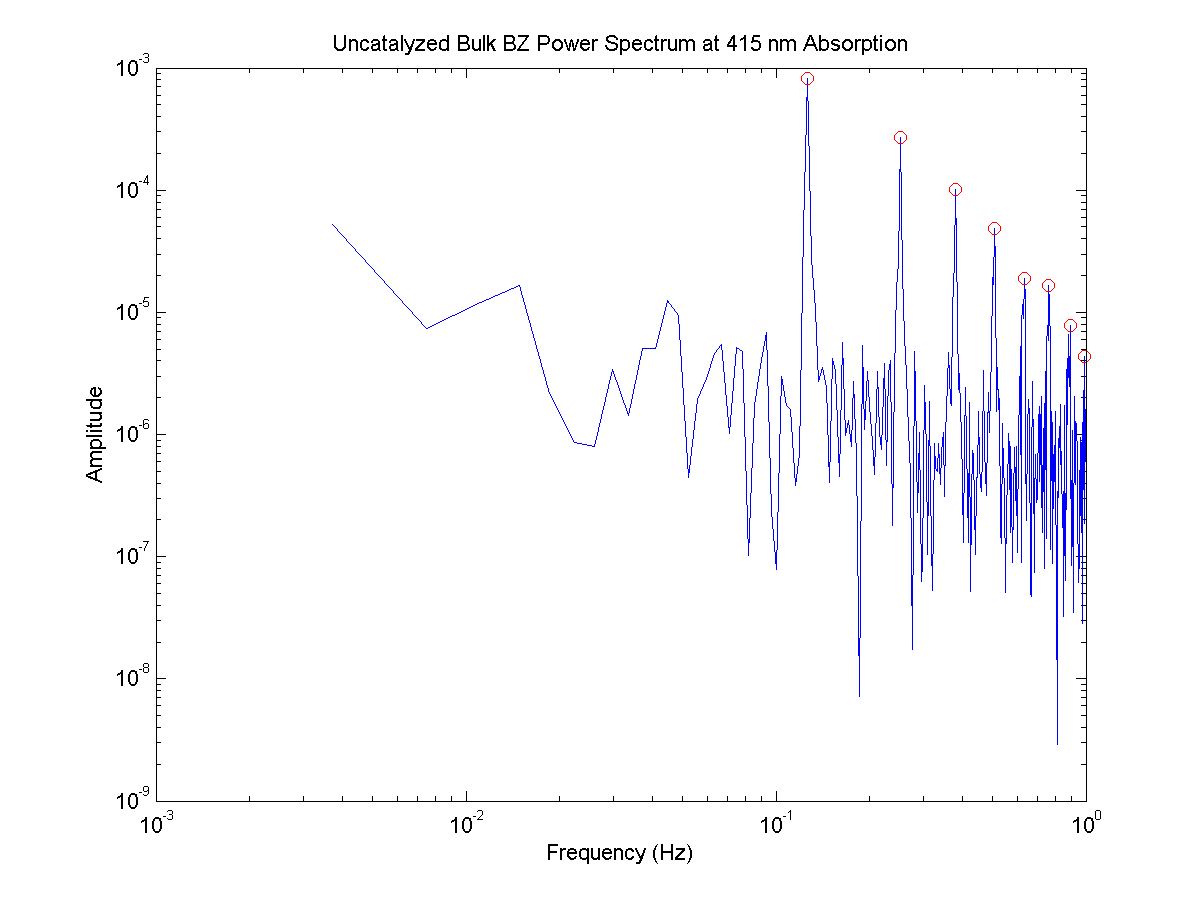
\includegraphics[width=0.8\textwidth]{frw415}
\centering
\caption{Power spectrum of the 415 nm time series for the uncatalysed bulk BZ 
reaction with irregular spikes marked.}
\label{ftw415}
\end{figure}

The frequencies of the marked spikes for the spectrum in \ref{ftw415} are 0.126 Hz,
0.253 Hz, 0.379 Hz, 0.506 Hz, 0.632 Hz, 0.758 Hz, 0.888 Hz, and 0.993 Hz.

\begin{figure}[H]
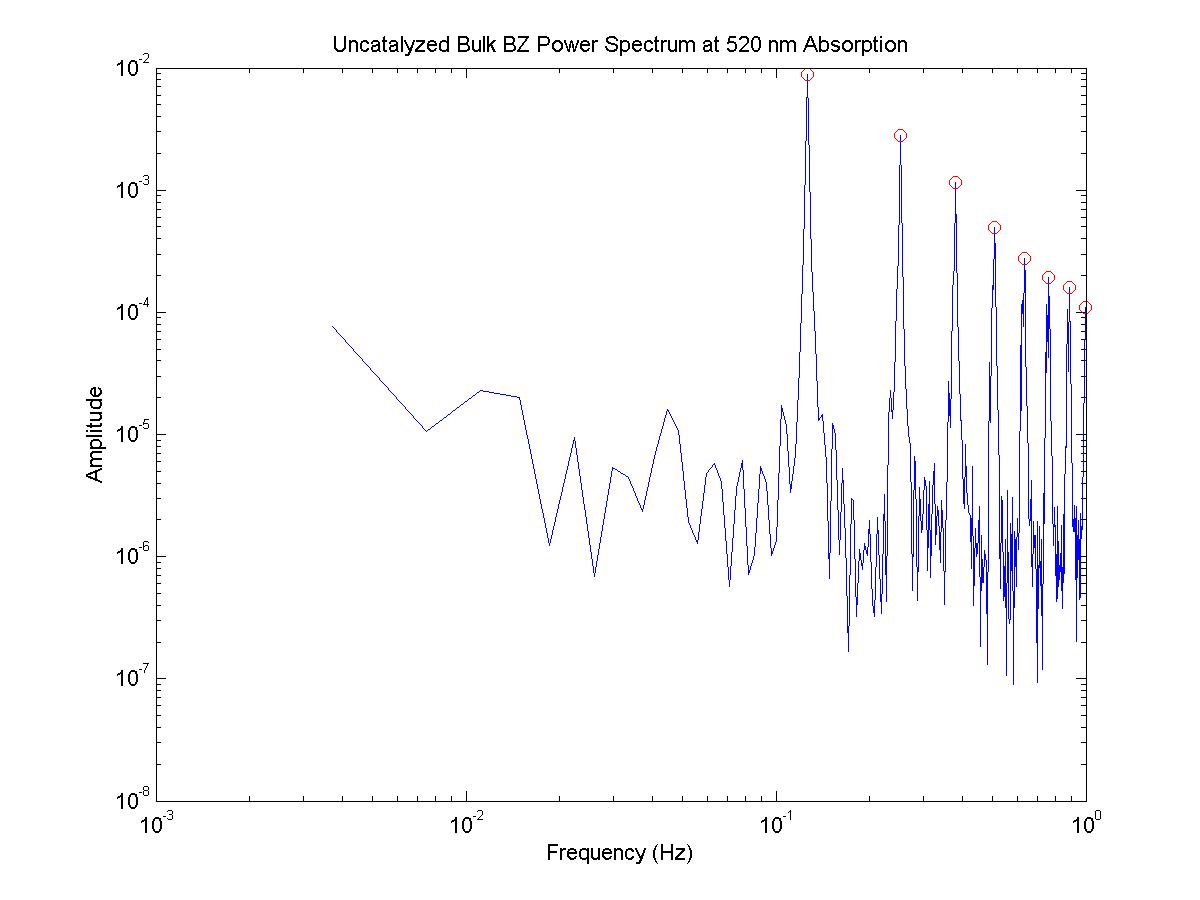
\includegraphics[width=0.8\textwidth]{frw520}
\centering
\caption{Power spectrum of the 520 nm time series for the uncatalysed bulk BZ 
reaction with irregular spikes marked.}
\label{ftw520}
\end{figure}

The frequencies of the marked spikes for the spectrum in \ref{ftw520} are
0.126 Hz, 0.253 Hz, 0.379 Hz, 0.506 Hz, 0.632 Hz, 0.758 Hz, 0.885 Hz, and 0.996 Hz.

\begin{figure}[H]
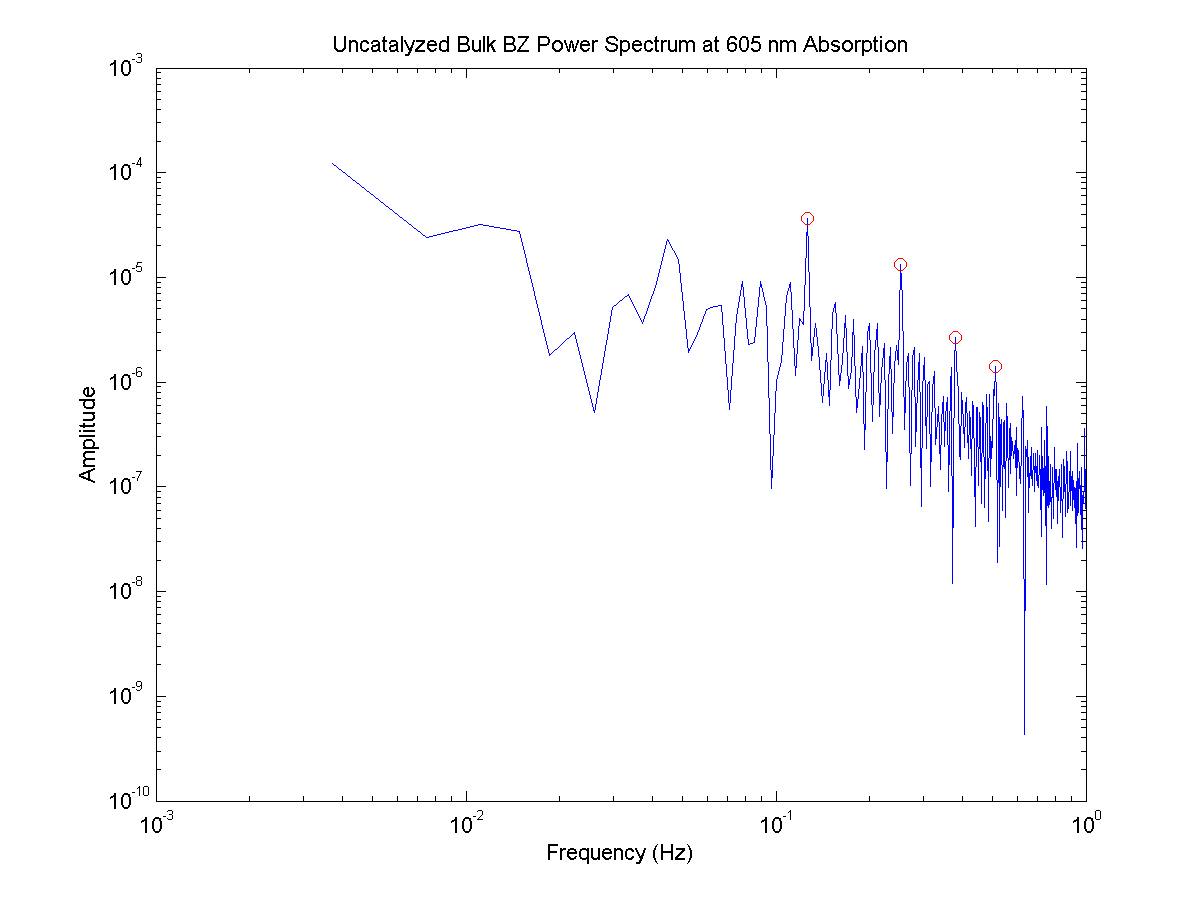
\includegraphics[width=0.8\textwidth]{frw605}
\centering
\caption{Power spectrum of the 605 nm time series for the uncatalysed bulk BZ 
reaction with irregular spikes marked.}
\label{ftw605}
\end{figure}

The frequencies of the marked spikes for the spectrum in \ref{ftw605} are
0.126 Hz, 0.253 Hz, 0.379 Hz, and 0.509 Hz.

All of the marker frequencies fall near integer multiples of the ``fundamental'' frequency
0.126 Hz, that is there appear to be ``open'' (they are integer, and not odd integer multiples)
overtones in the system.

\subsection{Thin-Layer (2-D) BZ Reaction}

\subsubsection{Wave Propagation via Fourier Decomposition}

Figure \ref{com} suggests the passage of seventeen wavefronts over the 402 second 
measurement,  giving an estimate of 42.2 mHz as the predominant frequency. Blips at
47.2 mHZ appear in the power spectra for both areas A and B  and are marked in Figures 
\ref{compowa} and \ref{compowb} below.

\begin{figure}[H]
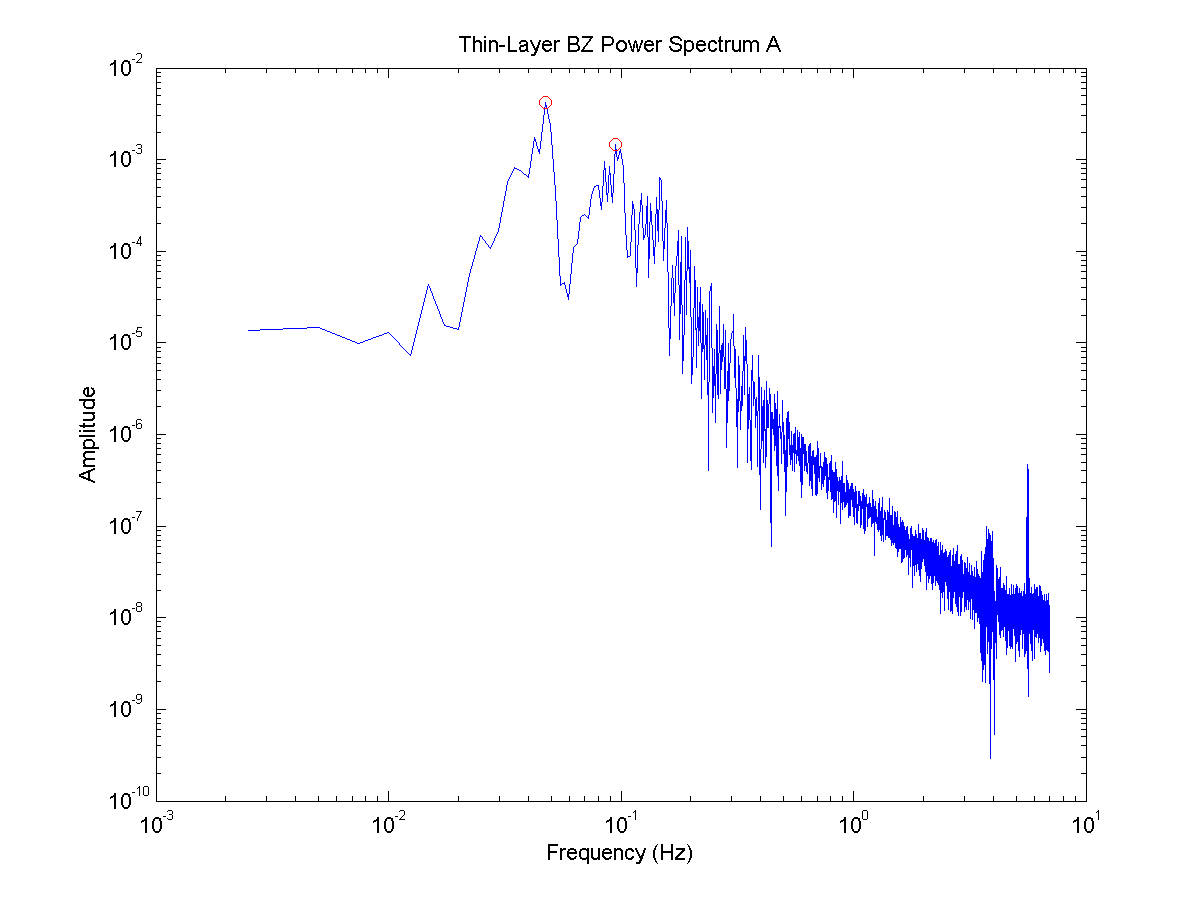
\includegraphics[width=0.8\textwidth]{frcoma}
\centering
\caption{Power spectrum of the time trace of A for the thin-layer BZ reaction with irregular
spikes marked.}
\label{compowa}
\end{figure}

\begin{figure}[H]
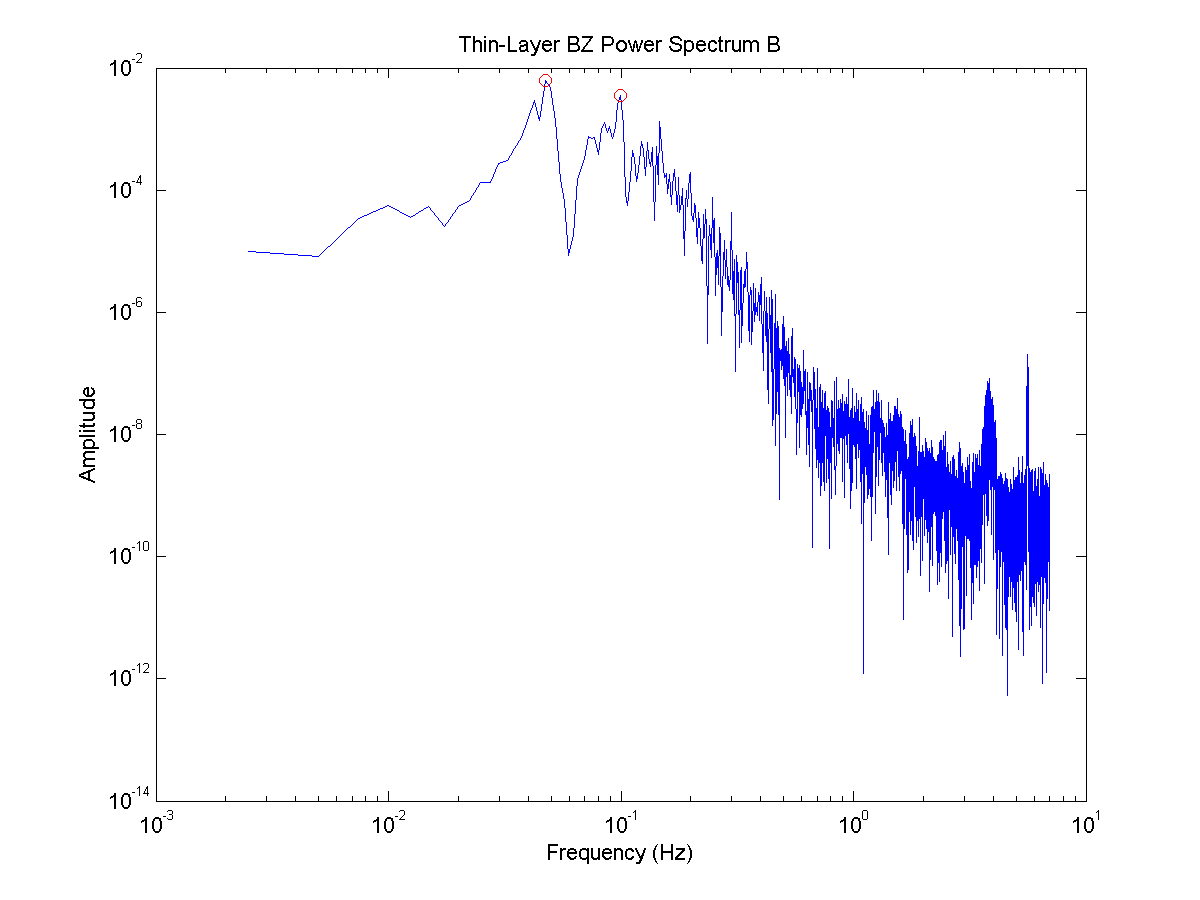
\includegraphics[width=0.8\textwidth]{frcomb}
\centering
\caption{Power spectrum of the time trace of A for the thin-layer BZ reaction with irregular 
spikes marked.}
\label{compowb}
\end{figure}

Of course, these frquencies only give the number of wavefronts passing A or B per unit 
time. We need the distance from A to B and the time between wavefront passages to get a 
velocity.

Watching the video recorded with the CMOS camera again, we seem the passage of a light
front, corresponding to the increased transmittance of 488 nm green light, across the screen
from B to A in a period of about six seconds, interspersed with a longer period of darkness,
corresponding to low transmittance of 488 nm green light. Looking again at Figure 5, we
understandt why the red spikes for B come so much closer to the following blue spikes for A,
rather than the preceeding. With this information, we can query the time between consecutive
spikes, i.e. wavefronts. Now understanding which spikes correspond to the same wavefront,
we can query the distance between the unadjusted center of mass spikes to get an estimate 
of the distance from A to B.

The average time for passage of a wavefront from B to A over seventeen wavefronts is
6.36 seconds with a standard of deviation of 0.83 seconds. The average distance between
the wavefront spikes at B and A over seventeen wavefronts is 147.38 $\mu$m with a 
standard of deviation 0.02 $\mu$m. This gives an average velocity with less than 2\% 
uncertainty of 23.2 $\mu$m per second.

\subsubsection{Theoretical Wavefront Velocity}

It has been experimentally determined by Field and Noyes that the wavefront velocity is 
related to the hydronium and bromate concentrations as
\begin{equation}
\mathrm{v}=\mathrm{k} [\mathrm{H}^+]^{1/2} [\mathrm{BrO}_3^-]^{1/2},
\end{equation}
where the rate constant
$\mathrm{k}$=0.04 cm sec\textsuperscript{-1} M\textsuperscript{-1}.
Further, the wavefront the result of the diffusion of concentration gradients, so its
propagation depends on the directions available for diffusion. The result of this is that in
thin-layer solution, the velocity of a wavefront initiated at a point depends on curvature as
\begin{equation}
\mathrm{v}^*=\mathrm{v}+\mathrm{D}\mathrm{K},
\end{equation}
where $\mathrm{D}$ is the diffusion coefficient on the order of $10^{-5}$ 
cm\textsuperscript{2} sec\textsuperscript{-1}, and $\mathrm{K}=\pm \mathrm{r}^{-1}$,
positive for a contracting wave and negative for expanding. Now, we have approximated the
distance between A and B assuming linear propagation of the wavefront, neglecting the 
curvature. This should be of little harm as long as we correctly assigned the wavefronts.

Using equations (16) and (17) with the concentrations from the procedure above, the 
given values for the rate and diffusion coefficients, and taking $\mathrm{r}\approx$ 3 cm
for a 60 mm perti dish, we calculate a velocity of 135 $\mu$m per second. There is an 
order of magnitude discrepancy between the two wavefront velocities.

\section{Discussion}

\subsection{Oscillatory Kinetics}

Neither by looking at the power spectra, nor by looking at the data in Figure \ref{tsun} am
I able to discern a damper in the bulk reaction. Thus, I cannot come up with a relaxation 
time. Further, since I see no damping, I do not know if after the reaction has reached 
equilibrium (which I know it must by the Second Law of Thermodynamics), if the reaction can 
be  regenerated. It would certainly be novel if there was a much lower frequency by which the
reaction appeared to damp to equilibrium, but then regenerated itself, or if it reached
steps of equilibrium and  the intermediates just needed to be perturbed between each step
to get the reaction to progress. The same goes for the thin-layer reaction, though in all 
likelyhood if I had simply observed the reaction for longer, I would have seen some damping
as the wavefronts interfered with each other. This holds even though the waves would have 
reinforced each other at some points; the thin layer solution was not controlled enough for 
us to get, say, diffraction patterns, though that would be cool to try.



\subsection{Wave Phenomena}

There is an  order of magnitude discrepancy between the wavefront velocity calculated from 
theory. and from time trace data. Perhaps in the theory we have made an assumption about
the diffusion that we shouldn't have. We need to account for the diffusion of intermediates
down their concentration gradients. If these gradients point in opposite directions for two
different intermediates, then maybe we should not simply concatenate equations (16) and 
(17).

The propogation of the BZ reaction wavefront in thin-layer solution depends upon 
the diffusion of particles down concentration gradients into a position to produce
sufficient inhomogeneity of particles and also to bring reacting species together. These are
not simple waves. Similarly, waves in water depend upon the diffusion of particles affected
by different forces like hydrogen bonds, forces from other dissolved particles, and
inhomogeneities in pressure and temperature. Though propagation speed in light waves may
be determined from wavelength and the media through which it passes, water and BZ waves
are the media, and therefore are not so simple. This is likely why they dissipate the way they
do; self interference damps things out. This is also probably why I have never seen a 
standing wave in water, and suggests that a perturbation of some sort is absolutely 
necessary to regenerate the BZ reaction if it damps to equilibrium.

\subsection{Conclusions}

This lab has emphasized the parallels between the chemical and physical as
schema and not just natural phenomena. The concept of waves and oscillations in a chemical
reaction that I can actually see suggests new ways to think of complex processes like the 
rolling of the ocean waves.

It would be fun to try to pass a thin-layer BZ wavefront through a diffreaction grating to see 
if we could get a distinct interference pattern.

%\begin{figure}[H]
%\includegraphics[width=0.8\textwidth]{filename}
%\centering
%\caption{Words.}
%\label{name}
%\end{figure}

%\begin{thebibliography}{9}

%\bibitem{}
%Last, F. I.; Surname, G. N. Title of Article. 
%\textit{Journal Title} [Online] \textbf{Year}, edition, page-page.

%\end{thebibliography}

\end{document}